\documentclass[12pt,a4paper]{scrartcl}

%\usepackage{algorithmic}    % Typesetting for pseudocode
%\usepackage{algorithm}      % Formatting for general algorithm blocks
\usepackage{fancyhdr}       % Gives fancy header
\usepackage{mdwlist}        % List related commands
\usepackage{url}            % Nicer URL formatting
\usepackage{new3151defs}    % COMP[39]151 defs
\usepackage{fancyvrb}

% Automata package
\usepackage{tikz}
\usetikzlibrary{arrows, automata, positioning, shapes}

% Page header
%\pagestyle{fancy}
%\lhead{COMP[39]151 Warmup Assignment
%\rhead{Timothy Wiley, z3109831}

% Line spacing 1.6 for 'double'
%\linespread{2}

% Declare commonly used graphic extensions and precedence
\DeclareGraphicsExtensions{.pdf,.png,.jpg}

\begin{document}

\title{COMP[39]151 Assignment 2}
\author{Aditya Keswani (z3242379) \\ 
        \texttt{akeswani@cse.unsw.edu.au} \\ 
        and \\ 
        Timothy Wiley (z3109831) \\
        \texttt{timothyw@cse.unsw.edu.au} }

\maketitle

\tableofcontents

\section{Definitions and Assumptions}
In order to implement the \emph{Life Stories Exchange} system, we make use of the following definitions and assumptions:
\begin{itemize}
    \item The total number of seniors, denoted as $nSeniors$, is known by all seniors.
    \item Each senior is assigned a unique id, denoted as $id$, in the range $[1,nSeniors]$
    \item Each senior knows the id's of all other seniors they are connected to.
          The predicate $conn(x,y)$ is true iff:
          \begin{itemize}
              \item Senior $x$ is permitted to share life stories with senior $y$, and
              \item Senior $x$ or $y$ is not dead, and
              \item Senior $x$ or $y$ is not talking to another senior $z$ where $z \notin \{x,y\}$.
          \end{itemize}
          Therefore, as our algorithm executes the value of $conn(x,y)$ may change.
    \item For each ordered pair of connected seniors $(x,y)$ there exists a one-directional message passing channel, $Chan(x,y)$, where senior $x$ sends to senior $y$.
          Therefore, two message passing channels exist between each pair of connected seniors.
\end{itemize}

\section{Description of Algorithm}
Our algorithm uses a round-based system.
Each round iterates through two phases:
\begin{enumerate}
    \item A phase of sending, and
    \item A phase of receiving.
\end{enumerate}

In the sending phase, each senior sends one message, $sendMsg$, to every connected senior with a lower id.
That is:
\begin{equation}
    \forall i, 0 \le i < id, conn(i, id) \quad C(id,i)!sendMsg
\label{eq:send-phase}
\end{equation}

In the receiving phase, each senior receives one message, $recvMsg$, from every senior they are connected to.
Also, each senior must respond, with $respMsg$, to any received message that was sent in the sending phase.
That is:
\begin{align}
    \forall i, 0 \le i \le nSeniors, conn(i, id) &\quad C(i,id)?recvMsg \\
    \forall i, 0 \le i, id < i \le nSeniors, conn(i, id) &\quad C(id,i)!respMsg
\label{eq:recv-phase}
\end{align}

The rounds continue until all seniors are sharing life stories, dead or having a seniors moment.
This sending/receiving process ensures that:
\begin{itemize}
    \item Only one message is send between pairs of connected seniors in the sending phase
    \item Seniors must receive a message from every connected senior.
    \item Seniors do not send to or try to receive from seniors that are dead or already sharing life stories.
\end{itemize}
We exploit these properties for our negotiation protocol and for detecting death.

The explanation of the remainder of our algorithm is broken into three components, the negotiation protocol, the senior state machine, and death detection.

\subsection{Negotiation Protocol}
Our protocol to determine which seniors share their life stories is based on the TCP-handshake protocol.
This protocol operates on a pair of seniors $x$ and $y$, with three phases:
\begin{enumerate}
    \item Senior $x$ sends a \emph{request} to senior $y$, which indicates they wish to share their life story.
    \item Senior $y$ responds with an \emph{acknowledgement}, indicating they accept the proposal.
    \item Senior $x$ establishes the sharing by responding with a \emph{confirmation}.
\end{enumerate}

If the three messages are sent, then the two seniors are considered to be sharing life stories.
However, at stages 2 and 3, the seniors may also send a \emph{decline}, indicating they are no longer interested in sharing stories.
Seniors also send a broadcast \emph{finish} message to indicate they are talking to someone else already.
The \emph{finish} messages are also used by seniors to update their $conn(id,y)$ values.

In summary, five types of messages can be sent:
\begin{itemize}
    \item \texttt{MSG\_REQ} - Request to talk
    \item \texttt{MSG\_ACK} - Acknowledge a request to talk
    \item \texttt{MSG\_CONF} - Confirm talking
    \item \texttt{MSG\_DECL} - Decline any request or acknowledgement
    \item \texttt{MSG\_FIN} - The senior is finished and will process no further messages.
\end{itemize}

\subsection{Senior State Machine}
We use a state machine to model the how the stages of the message protocol impact the behaviour senior, shown in Fig. \ref{fig:senior-state-machine}.
The red states and transitions represent the sending phase of the message protocol, while the blue states and transitions represent the receiving phase.
The notation $x!\texttt{MSG}$ and $x?\texttt{MSG}$ is shorthand for sending and receiving from senior with id $x$ (for example $x!\texttt{MSG}$ expands to $Chan(id,x)?\texttt{MSG}$)

\begin{figure}[h]
   \centering
   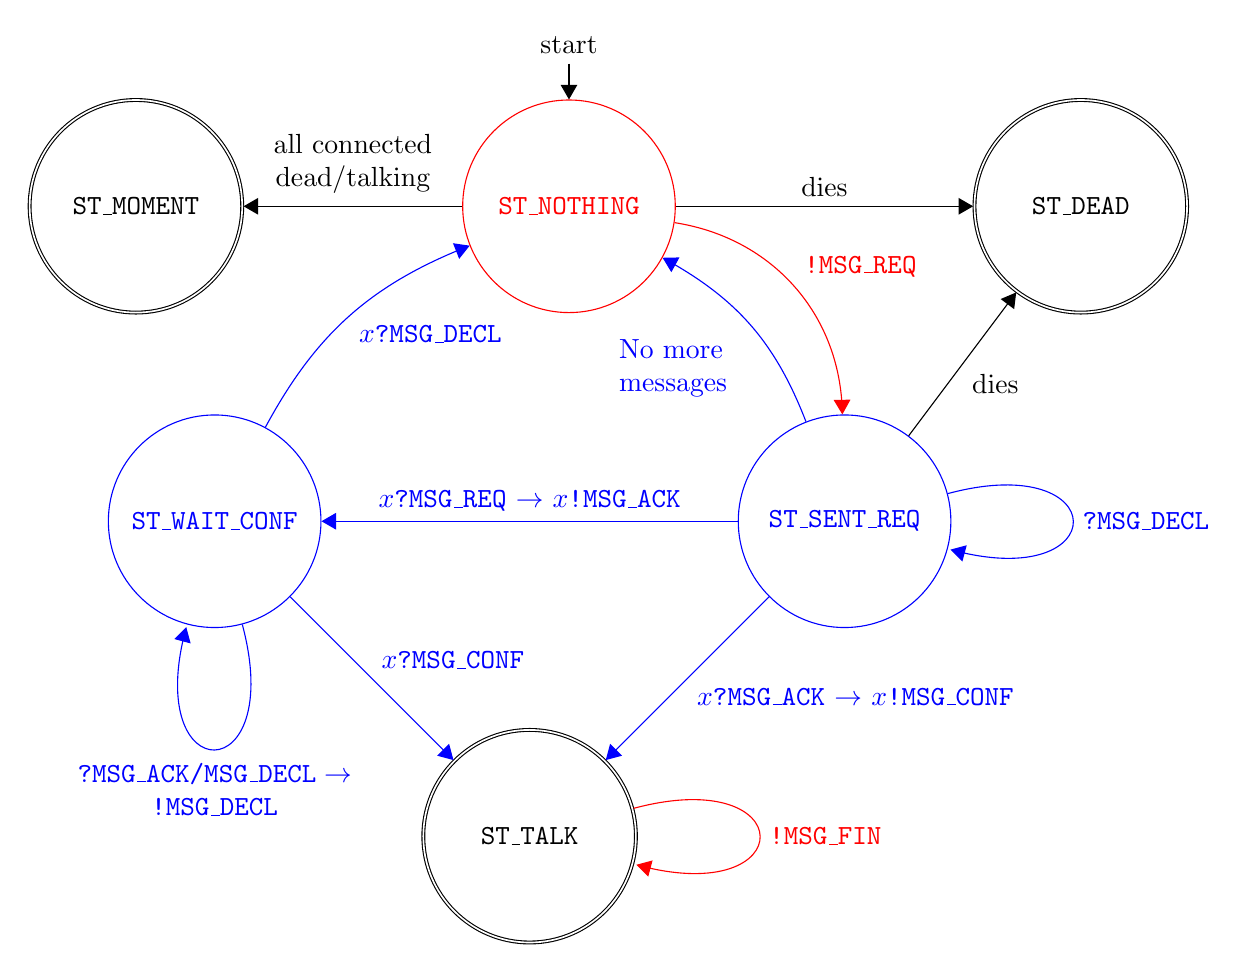
\begin{tikzpicture}[->,>=triangle 60, on grid,auto]

   % Nodes
      \node[state,initial above,minimum size=2.7cm,color=red]    (noth)  at (4.5,8)   {\texttt{ST\_NOTHING}};
      \node[state,accepting,minimum size=2.7cm]        (talk)  at (4,0)     {\texttt{ST\_TALK}};
      \node[state,accepting,minimum size=2.7cm]        (dead)  at (11,8)    {\texttt{ST\_DEAD}};
      \node[state,accepting,minimum size=2.7cm]        (momt)  at (-1.0,8)  {\texttt{ST\_MOMENT}};
      \node[state,minimum size=2.7cm,color=blue]                  (sreq)  at (8,4)   {\texttt{ST\_SENT\_REQ}};
      \node[state,minimum size=2.7cm,color=blue]                  (wcnf)  at (0.0,4)     {\texttt{ST\_WAIT\_CONF}};

   % Paths
      \path (noth) edge [bend left=00]  node[above]       {$\begin{array}{c} \textrm{all connected} \\ \textrm{dead/talking} \end{array}$} (momt)
                   edge [bend left=00]  node[above]       {dies} (dead)
                   edge [bend left=40,color=red]  node[above right] {\texttt{!MSG\_REQ}} (sreq);
      \path (sreq) edge [bend left=00]  node[below right] {dies} (dead)
                   edge [loop right,color=blue]    node[right]       {\texttt{?MSG\_DECL}} (sreq)
                   edge [bend left=00,color=blue]  node[above]       {$x$\texttt{?MSG\_REQ} $\rightarrow$ $x$\texttt{!MSG\_ACK}} (wcnf)
                   edge [bend right=20,color=blue] node[below left]  {$\begin{array}{l} \textrm{No more} \\ \textrm{messages} \end{array}$} (noth)
                   edge [bend left=00,color=blue]  node[below right] {$x$\texttt{?MSG\_ACK} $\rightarrow$ $x$\texttt{!MSG\_CONF}} (talk);
      \path (wcnf) edge [bend left=00,color=blue]  node[above right] {$x$\texttt{?MSG\_CONF}} (talk)
                   edge [loop below,color=blue]    node[below]       {$\begin{array}{c}\texttt{?MSG\_ACK/MSG\_DECL} \rightarrow \\ \texttt{!MSG\_DECL} \end{array}$} (wcnf)
                   edge [bend left=20,color=blue]  node[below right] {$x$\texttt{?MSG\_DECL}} (noth);
      \path (talk) edge [loop right,color=red]    node[right]       {\texttt{!MSG\_FIN}} (talk);
   \end{tikzpicture}
   \caption{Senior State Machine}
   \label{fig:senior-state-machine}
\end{figure}

The state \texttt{ST\_NOTHING} in the default state to which the senior returns if there are no messages to respond to.
This is also the starting point for the sending phase. Once all messages have been sent, the senior enters \texttt{ST\_SENT\_REQ} to perform the receiving phase.
In this state, the following properties are observed:
\begin{itemize}
    \item Messages are received concurrently from all connected seniors.
    \item Received messages are processed sequentially.
    \item The first message that matches one of the valid transitions, causes the senior to change state, but the receiving process continues until completion.
          That is, until a message has been received from every connected senior.
          This is why the state \texttt{ST\_WAIT\_CONF} may receive requests or acknowledgements and needs to send declines in response to them.
\end{itemize}

If the senior transitions into \texttt{ST\_WAIT\_CONF}, then it records the id of the senior which caused the transition, recorded in the variable $x$.
Only receiving a decline or confirmation from senior $x$ will cause a transition out of the waiting state.
Whereas messages from other seniors are rejected.

It should be noted that the sending of the broadcast \texttt{MSG\_FIN} constitutes part of the sending phase.
This is because such messages will not be received until the next receiving phase after they have been sent.
Also, the receiving of these messages is not recorded on the diagram, but it is assumed they do not cause any state transition.

The points at which seniors can die are also strictly maintained.
Seniors cannot die when in the state \texttt{ST\_WAIT\_CONF} as they may not send another message once in this state.
Also, our implementation must ensure that if a senior is to die it does so before entering the state \texttt{ST\_WAIT\_CONF}.

Finally, it should be noted that the state machine ensures that any senior sends an extra \texttt{MSG\_CONF} or \texttt{MSG\_DECL} whenever a connected senior responds their request with an acknowledgement.

\subsection{Death Detection}
To detect death we exploit two properties of our solution:
\begin{itemize}
    \item For each valid channel $Chann(x,y)$ at least one message is sent along it each round.
    \item Reading of messages is performed concurrently
\end{itemize}

Therefore, we place a timeout on reading from a channel.
If this timeout occurs before a message is received, then we can immediately infer the senior we are attempting to receive from has died.

Once a timeout has been detected, the senior updates their value for $conn(id,y)$ so that they are no longer connected to the dead senior.

It should be noted that we need to make the timeout large enough to ensure every senior has the opportunity to send their messages.
Also, while messages are received concurrently, they are processed sequentially.
This means we must allow time for the sequential processing to ensure seniors have adequate time to respond.

\section{Verification}
\label{sec:verification}
We have verified our C implementation using, where possible, a faithful conversion to Promela, with a set of assertions and LTL's.
The differences between our C and Promela implementation are:
\begin{itemize}
    \item The number of seniors is set by the \texttt{N\_SENIORS} define (line 1).
    \item We model the allowable connectivity (ie. sharing of life stories) between seniors using Promela's non-determinism (lines 313-335).
          We generally verify our properties on fully connected graphs, which can be enabled by setting $\texttt{FULLY\_CONN} = 1$,
            as using any type of graph creates a blowout in the state-space.
    \item We model the ability of seniors to die using Promela's non-determinism (lines 157-160).
          Death can be disabled by setting $\texttt{CAN\_DIE} = 0$
    \item Where a senior that must die has the option to die or send a message, we model this using Promela's non-determinism (lines 198-202).
    \item We model death detection by having seniors that have died send a broadcast \texttt{MSG\_FIN} after death.
          This is identical to seniors that have started talking.
          This is an appropriate compromise, since in the C implementation when a timeout occurs, the received message is set to \texttt{MSG\_FIN}.
\end{itemize}

We verify two key properties:
\begin{itemize}
    \item Termination of all seniors.
    \item Valid final connections of seniors (safety).
\end{itemize}
We also consider the number (or degree) of deaths our algorithm can cope with.

For verifying our LTLs and asserts we use all combinations of $\texttt{N\_SENIORS} \in \{3, 4 5\}$, $\texttt{FULLY\_CONN} \in \{0, 1\}$ and $\texttt{CAN\_DIE} \in \{0, 1\}$.
We use fully connected and no death as this drastically reduces the state space search.
We also then enable dieing.
If LTL's do not cause errors both of these tests (for the ranges of \texttt{N\_SENIORS}) we consider them proven, as removing connections from the graph does not provide any additional information.
We do test with non-fully connected graphs but for 4 or more seniors Promela is not able to search much of the state space, so this is not as useful.

\subsection{Termination}
\label{sub:verify-term}
We prove termination by considering the number of seniors who have not reached a terminal state (see Fig. \ref{fig:senior-state-machine}).
We will show that on each round (of sending and receiving) this number always decreases, hence every senior, and the entire protocol must eventually terminate.
We also assume weak fairness to ensure that no senior stalls.

By inspection of the state machine, we can see that seniors choose to die, which is a terminal state.
Inspection also shows seniors may have seniors moments if all values of $conn(id,y)$ are false.
Thus trivially, seniors may terminate on any round.

We therefore, consider the case of $n$ seniors, where no senior may die, and without loss of generality, where the seniors are fully connected.
Now consider the messages, \texttt{MSG\_REQ}, sent in the sending phase of a round.
Fig. \ref{fig:termination-n4}, shows an example setup for $n = 4$.
\begin{figure}[h]
   \centering
   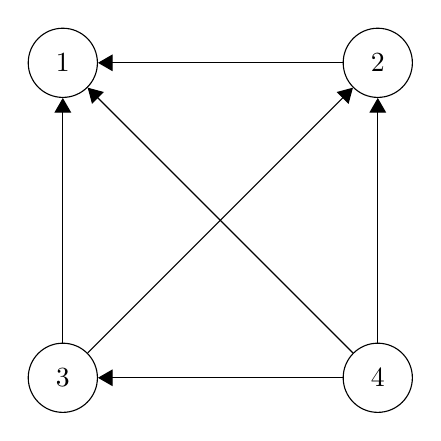
\begin{tikzpicture}[->,>=triangle 60, on grid,auto]

   % Nodes
      \node[state]  (p1)    at (0,4)    {$1$};
      \node[state]  (p2)    at (4,4)    {$2$};
      \node[state]  (p3)    at (0,0)    {$3$};
      \node[state]  (p4)    at (4,0)    {$4$};

   % Paths
      \path (p4) edge [bend left=00]  node[above]       {} (p3)
                 edge [bend left=00]  node[above]       {} (p2)
                 edge [bend left=00]  node[above]       {} (p1);
      \path (p3) edge [bend left=00]  node[above]       {} (p2)
                 edge [bend left=00]  node[above]       {} (p1);
      \path (p2) edge [bend left=00]  node[above]       {} (p1);
   \end{tikzpicture}
   \caption{Messages sent in sending phase of a round for 4 fully connected seniors}
   \label{fig:termination-n4}
\end{figure}

Consider the senior with the highest id $n$.
They have sent a \texttt{MSG\_REQ} to every other senior they are connected to.
There are two cases:
\begin{itemize}
    \item By inspection of the state machine, if any one of those seniors ($id = 1 \ldots n-1$) reply with a \texttt{MSG\_ACK}.
          senior $n$ and the responding senior must both enter \texttt{ST\_TALK}, and share stories with one another.
    \item If all seniors $id = 1 \ldots n-1$ respond with \texttt{MSG\_DECL}, then senior $n$ does not impact on the protocol, and can be ignored.
          We can then repeat the reasoning as if there were only $n-1$ seniors.
\end{itemize}

By induction, either two seniors enter \texttt{ST\_TALK} or the case where $n=2$ is reached, shown in Fig. \ref{fig:termination-n2}.
\begin{figure}[h]
   \centering
   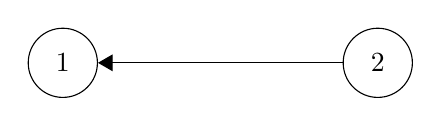
\begin{tikzpicture}[->,>=triangle 60, on grid,auto]

   % Nodes
      \node[state]  (p1)    at (0,0)    {$1$};
      \node[state]  (p2)    at (4,0)    {$2$};

   % Paths
      \path (p2) edge [bend left=00]  node[above]       {} (p1);
   \end{tikzpicture}
   \caption{Messages sent in sending phase of a round for 2 seniors}
   \label{fig:termination-n2}
\end{figure}

By executing the state machine, it can be seen these seniors must enter \texttt{ST\_TALK}.

We have therefore shown that in each round at least one senior must enter a terminal state.
Hence, all seniors must eventually terminate.

We verify this is promela using LTL's of the form:
\begin{equation}
    \Always(pstart \Implies \Eventually pterm)
\label{eq:ltl-term}
\end{equation}
where $pstart$ and $pend$ are labels at the start and end points of the senior code.
LTL's \emph{term1, term2} and \emph{term3} are samples.

\subsection{Safety properties}
There are 3 safety properties that need to be verified:
\begin{itemize}
    \item A senior that should die, eventually does,
    \item There cannot be two connected seniors having moments, and
    \item If senior $x$ thinks they are talking to senior $y$, then senior $y$ also thinks they are talking to senior $x$.
\end{itemize}

\subsubsection{Eventual Death}
We ensure seniors eventually die by:
\begin{itemize}
    \item If there are no messages to send, they do not have a moment instead they die,
    \item Before entering \texttt{ST\_WAIT\_CONF} a senior must die, and
    \item Before sending a \texttt{MSG\_CONF} a senior must die.
\end{itemize}

We also verify this condition in Promela with LTL's of the form
\begin{equation*}
    \Always(shouldDie[x] \Implies \Eventually(states[x] == \texttt{ST\_DEAD}) )
\label{eq:ltl-death}
\end{equation*}
where $shoudDie$ is an array indicating a given senior must eventually die, and $states$ is the current state-machine state of each senior.
That is, in all states, any senior that must die eventually has their state set to \texttt{ST\_DEAD}.
LTL's \emph{death1, death2} and \emph{death3} are samples.

\subsubsection{No Connected Moments}
To prove that two seniors who are able to share life stories with each other do no have senior moments,
    consider the case of two connected seniors in Fig. \ref{fig:termination-n2}.
By the reasoning in \ref{sub:verify-term}, if neither die, and do not think the other has died, then they will both enter \texttt{ST\_TALK}.
What remains to be shown is that neither will detect the other has died.

By inspection of Fig. \ref{fig:termination-n2}, Senior 1 will not detection senior 2 has died as senior 2 will send a message.
Also, by the state machine, senior 1 must eventually read the message from 2 and respond.
Therefore senior 2 will not detect senior 1 has died.
Thus, given sufficient time for the seniors to receive, process and respond to messages, death will not be detected.
This means two connected seniors cannot both be having moments.

We verify this in Promela with LTL's of the form:
\begin{equation}
    \Always(connections[x].b[y] \Implies \Not(states[x] == \texttt{ST\_MOMENT} \And states[y] == \texttt{ST\_MOMENT}))
\label{eq:ltl-moments}
\end{equation}
where $connections$ records if senior $x$ and $y$ can share life stories.
LTL's \emph{momnt1, momnt2} and \emph{momnt3} are samples.

\subsubsection{Reciprocal Talking}
The design of the senior state machine using a 3-way handshake and sequential processing of received messages gives the following properties:
\begin{itemize}
    \item A senior will only attempt to talk with one other senior in a single round.
    \item If there is any mis-match of expected messages a decline is always sent.
\end{itemize}

Thus, there cannot be a state where senior $x$ thinks they are talking to senior $y$, but $y$ is talking to $z$.
We verify this is Promela using LTL's of the form:
\begin{equation}
    \Always(talking[x] == y \Implies \Eventually(talking[y] == x))
\label{eq:ltl-recipricol}
\end{equation}
where $talking$ records who the senior believes they are talking to after they enter the state \texttt{ST\_TALK}.
LTL's \emph{talking1, talking2} and \emph{talking3} are samples.

\subsection{Degree of Death}
Our implementation is able to cope with any number of seniors dieing.
By modeling death in Promela using non-determinism, all combinations of ways seniors can die is covered.
As our termination and safety conditions all verify without error, we are therefore able to cope with any ordering and combination of death.

\section{Complexity Analysis}
The following facts are used in the complexity analysis:
\begin{itemize}
    \item As noted in section \ref{sub:verify-term}, at worst, one senior will enter an end state on each round.
    \item Therefore, given $n$ seniors, there will be at most $n$ rounds.
    \item Also in each round, each senior receives $k-1$ messages, where $k$ is the number of remaining seniors.
\end{itemize}

\subsection{Message Complexity}
In each round, at worst, $(k-1)^2 = O(k^2)$ messages a sent amongst the remaining seniors.
Given at most $n$ round, the message complexity is $\sum_{i=1}^n (i-1)^2$, which is $O(n^3)$

\subsection{Time Complexity}
As the workload is a constant factor of the number of messages received, $O(k)$ work is done by each senior, making $O(k^2)$ work done per round.
Therefore, given at most $n$ rounds, the total Time Complexity is $O(n^3)$

\end{document}
